\chapter{Simulation}
The activities of the simulation is described in this chapter.
An overview of NS-3 is given, which is then followed by the actions taken, setup
used, assumptions made and overall explanation of the simulation.

\section{NS-3}
A discrete event network simulator, NS-3 is used extensively in network research
and education. The workings and performance of packet data network are modelled
and NS-3 provides a platform for the simulation and experimentation of various
packet-based research. C++ and Python are the predominant language in which NS-3
is written with \textit{waf} as the build system. Design of NS-3 capitalizes on
the object oriented nature of these languages\cite{nsonline}.\\\\
There are various components of packet-based network, fundamentally there are the
endpoint devices, routers,NIC devices ,switches and the medium of exchange.
These components,however in NS-3, are abstracted to reflect what the components
actually do. The endpoint devices are called \textit{Nodes}, exchange medium
- \textit{Channel} and the applications that are generating the packets are 
\textit{Applications} just to name a few. The file/folder structure of a simulation
consist of a model which depicts the fine details of the simulation, a helper that
is supposed to include files containing the installation helper functions, an 
example folder to implement an example of the simulation. There are also doc and 
tests folders and the just as their names suggest they hold documentation and tests
files.\\\\
Installation of the NS-3 is not needed to get a simulation running, as the examples 
or experiments can be run using the binary files gotten from the build process.
It is actually not recommended to do installation of NS-3. Installation in this case
refers to running the command \textbf{\textit{./waf install}}.

\section{Setup}
The simulation was performed on a Gentoo Linux flavor computer with a 64 bit Intel
Eight-Core processor with model name \textit{Intel(R) Core(TM) i7-8565U CPU @
1.80GHz} and RAM of 32GB. Version 3-30 of NS-3 provided the platform on which to
undertake the research. At the time of setting up, this version was the latest most
stable release.\\\\
NS-3 is a voluminous software, the faster processor is needed, as a change to any
file would mean rebuilding the file and its dependencies and those that depend on it.
The version is also critical. Most versions are not backward compatible hence what
works on 3.29 might not work on 3.30 without a little tinkering.\\\\
Gentoo Linux, even though time consuming and quite advance in installation and
setting up, turns to be one of the fastest linux operating systems available. This is
partly due to the fact that source codes are compiled on the host computer with 
specific flags set for optimality.

\section{Components}
For a data packet to move from one endpoint to another, there are components such as,
the packet generating and receiving nodes which will have NIC, the medium(s) through
which the packet traverses also forms a part of the components.\\\\
There are three critical parts, worth mentioning for this simulation; the header which
is attached to the packet, tag-augmented sensor devices and the reader, which, in this
case, is augmented with a server.\\\\
A discussion of the various components follow next.
\subsection{Packet Header}
Various parts of a packet header which is added to a payload enable the packet to get
to its intended destination. A 4-byte(32 bits) header was created, having two fields
of 16 bits each representing the packet type being sent: data packet or broadcast 
and the state of the tag augmented sensor: whether a new data is available for 
transmission or not.\\
\begin{figure}[h!]
\begin{tikzpicture}
    \tikzumlset{font=\tiny\ttfamily}
    \umlemptyclass[x=0,y=0]{Header}{
}{}
\umlclass[x=5.5,y=-2]{AptMacHeader}{
  -m\_id : uint16\_t \\ -m\_type : uint16\_t \\ -m\_stateChange : uint16\_t \\
  -m\_dataLoss : uint16\_t
}{
  +AptMacHeader() \\ +SetId(id : uint16\_t) : void \\ +GetId (void) : const
  uint16\_t\\ +SetPacketType(ptype : uint16\_t) : void \\ +GetPacketType(void) :
  const uint16\_t \\ +SetStateChange(stateChange : uint16\_t) : void \\ 
  +GetStateChange(void) : const uint16\_t \\ \umlstatic{+GetTypeId(void) : TypeId}\\
  +GetDataLoss(void) : const uint16\_t \\ +SetDataLoss(d : uint16\_t) : void \\
  \umlvirt{+Serialize(start : Buffer::Iterator) : const void} \\
  \umlvirt{+Deserialize(start : Buffer::Iterator) : uint32\_t} \\
  \umlvirt{+GetSerializedSize(void) : const uint32\_t} \\
  \umlvirt{+GetInstanceTypeId (void) : const TypeId} \\
  \umlvirt{+Print(\&os : std::ostream) : const void}\\
}
\umlenum[x=11.5,y=-4]{HeaderContents}{
    BROADCAST : uint16\_t \\ DATA : uint16\_t \\ STATECHANGE : uint16\_t
}

%\umlassoc[geometry=-|-, arg1=tata, mult1=*, pos1=0.3, arg2=toto, mult2=1, pos2=2.9, align2=left]{C}{Header}
%\umlunicompo[geometry=-|, arg=titi, mult=*, pos=1.7, stereo=vector]{D}{C}
%\umlimport[geometry=|-, anchors=90 and 50, name=import]{sp2}{sp1}
\umlaggreg[geometry=-|]{AptMacHeader}{HeaderContents}
\umlinherit[geometry=-|]{AptMacHeader}{Header}
%\umlnote[x=2.5,y=-6, width=3cm]{B}{Je suis une note qui concerne la classe B}
%\umlnote[x=7.5,y=-2]{import-2}{Je suis une note qui concerne la relation d'import}
\end{tikzpicture}
\caption{Class Diagram - APT-MAC Header}
\label{fig:headerUML}
\end{figure}\\
The UML class diagram is illustrated in Figure \ref{fig:headerUML}. The \emph{
constructor, getter and setter} functions are for their usual purposes. \emph{
Serialize} function puts the various fields of the header in series by writing them
from host-order to network-order and the \emph{Deserialize} reads from network-order
to host-order. \emph{Enum HeaderContents} holds the value of the various fields of
the header.

\subsection{Tag Augmented Sensor Devices}
Devices in a smart home are broadly classified under three categories: periodic
(e.g., temperature sensors), real-time (e.g., joystick, cameras) and event based 
(e.g., presence detector, remote of appliances)\cite{Maselli}. The state changes
of the various devices were modelled according to Markov Chains\cite{Tolver}.\\
\begin{centering}
\begin{figure}[h!]
    \begin{subfigure}[b]{.5\textwidth}
        \centering
        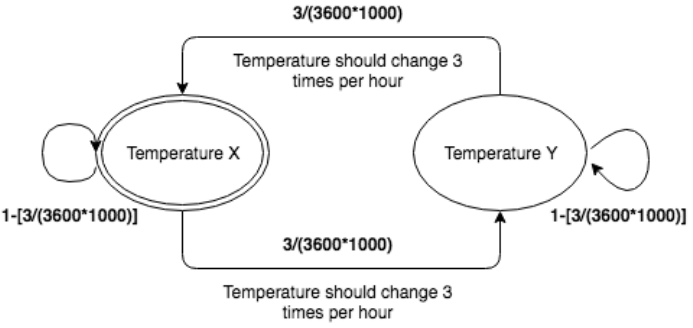
\includegraphics[width=1\linewidth]{temperature-sensor}
        \caption{Temperature Sensor model}
        \label{fig:temperature-sensor}
    \end{subfigure}
    \begin{subfigure}[b]{.5\textwidth}
        \centering
        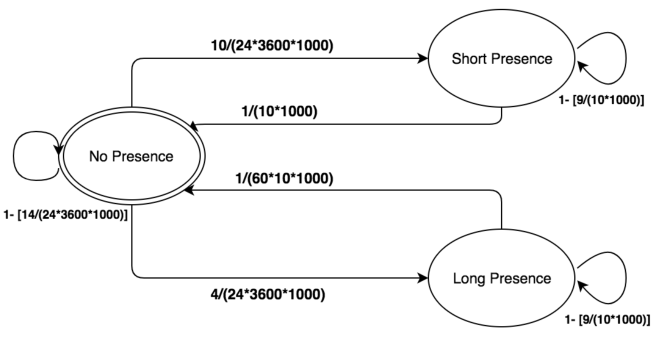
\includegraphics[width=1\linewidth]{presence-sensor}
        \caption{Presence Sensor model}
        \label{fig:presence-sensor}
    \end{subfigure}
    \begin{subfigure}[b]{.5\textwidth}
        \centering
        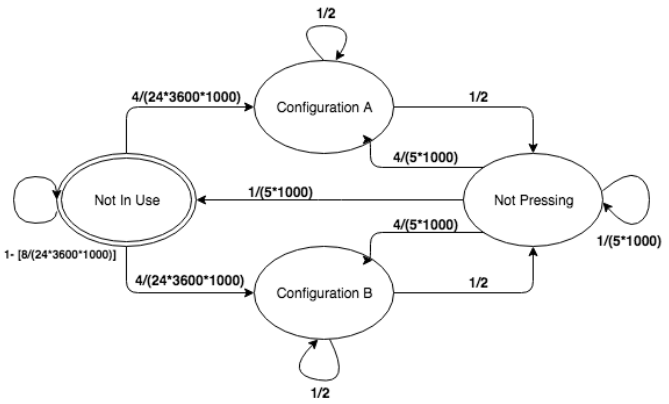
\includegraphics[width=1\linewidth]{tv-remote}
        \caption{TV Remote model}
        \label{fig:tv-remote}
    \end{subfigure}
    \begin{subfigure}[b]{.5\textwidth}
        \centering
        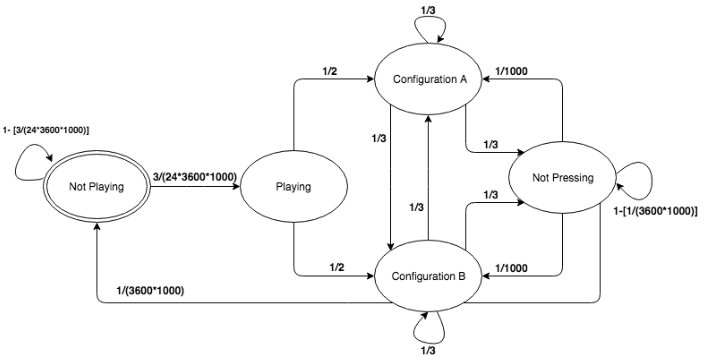
\includegraphics[width=1\linewidth]{joysick-sensor}
        \caption{Joystick model}
        \label{fig:joysick-sensor}
    \end{subfigure}
\end{figure}
\end{centering}\\
Figures \ref{fig:temperature-sensor} to \ref{fig:joysick-sensor}, taken from
\cite{Maselli}, depicts the transition probabilities of the various states a device
could be in. The state change is based on time. Taking fig \ref{fig:temperature-sensor}
for instance, it was found that a temperature sensor produces new data three times in
an hour hence the various probabilities with respect to time in milliseconds.
There are two states in with a temperature sensor and with a probability of 
$3/(3600*1000)$ it changes from, lets say, state X to Y or vice versa and with
$1-3/(3600*1000)$ stays in its state.\\\\
\begin{centering}
\begin{figure}[h!]
    \begin{tikzpicture}
        \tikzumlset{font=\tiny\ttfamily}
        \umlemptyclass[x=-3.5,y=0]{Application}{
        }{}
        \umlclass[x=2.5,y=-2]{SensorNode}{
            -m\_port : uint16\_t \\ -m\_PreState : uint16\_t \\
            -m\_socket : Ptr$\langle$Socket$\rangle$ \\
            -packetGenerationTime : uint64\_t \\ -m\_PreState : uint64\_t \\
            -m\_newDataCountSent : uint64\_t \\ -m\_newDataCountProduced : uint64\_t
            \\ -m\_queryCounter : uint64\_t \\ -dataLossLog : std::string \\
            -dataFile : std::string \\
            -m\_tagDataVector : std::vector$\langle$Ptr$\langle$NS3::Packet$\rangle$$\rangle$
            \\ -m\_delayVector : std::vector$\langle$uint16\_t$\rangle$ \\
            -m\_dllVector : std::vector$\langle$uint16\_t$\rangle$
        }{
        +SensorNode() \\
        \umlvirt{$\sim$SensorNode} \\
        \umlvirt{-StartApplication(void) : void} \\
        \umlvirt{-StopApplication(void) : void} \\
        \umlvirt{\#DoDispose(void) : void} \\
        -HandleBroadcast(socket : Ptr{\tiny$\langle$}Socket{\tiny$\rangle$}) :
        void \\
        -HandleDataQuery(socket : Ptr{\tiny$\langle$}Socket{\tiny$\rangle$})
        : void \\ -indexOfLargestProb({\tiny\&}matrix : Matrix) : int \\
        -GeneratePacket(void) : void \\
        -SchedulePacketGenerate(void) : void \\
        -MultMatrix({\tiny\&}trsMtx : const Matrix, {\tiny\&}trsMtxb
        : const Matrix) : Matrix \\ -NextState(currentTime : NS3::Time) : Matrix \\
        \umlstatic{+GetTypeId(void) : TypeId} \\ +Print({\tiny\&}a : const Matrix)\\

        +Send(socket : Ptr{\tiny$\langle$}Socket{\tiny$\rangle$} , from : NS3::Address , Packet : Ptr{\tiny$\langle$}Packet{\tiny$\rangle$}) \\
        +GetNewDataSent(void) : int64\_t \\ +SetNewDataSent(c : int64\_t) : void \\
        +UpdateNewDataSent(void) : void \\ +SetNewDataProduced(c : int64\_t)\\
        +GetNewDataProduced(void) : int64\_t \\ +UpdateNewDataProduced(void) : void
        \\ +UpdateQueryCounter(void) : void \\ +ResetQueryCounter(void) : void
        \\ +GetQueryCounter(void) : uint64\_t \\
        +AppendDataFile(filename : std::string , data : uint16\_t ) \\
        +CreateDatafile(device : std::string , devideID : uint32\_t)
    }
    \umltypedef[x=-1.5,y=-9]{Matrix}{}{}
    \umlemptyclass[x=-4,y=-3.5,template={T,U}]{std::vector}{}{
    }
    \umlclass[x=4.0,y=-9.5]{SensorNodeHelper}{
        -m\_factory : ObjectFactory \\
        -m\_server : Ptr{\tiny$\langle$}SensorNode{\tiny$\rangle$}
    }
    {
        +SensorNodeHelper() \\ +SensorNodeHelper(port : uint16\_t) \\
        +SetAttribute(name : std::string , {\tiny\&}value : const AttributeValue) \\
        +Install(c : NodeContainer) : ApplicationContainer \\
        +GetServer(void) : Ptr{\tiny$\langle$}SensorNode{\tiny$\rangle$}
    }
    \umlenum[x=9.5,y=-4.1]{HeaderValidation}
    {
        BROADCAST : uint16\_t \\ BROADCAST\_REPLY : uint16\_t \\ DATA : uint16\_t
        \\ DATA\_REPLY : uint16\_t \\ STATE\_CHANGED : uint16\_t \\
        STATE\_NOT\_CHANGED : uint16\_t
    }{}
    \umldep[geometry=-|]{Matrix}{std::vector}
    \umldep[geometry=-|]{SensorNode}{Matrix}
    \umlinherit[geometry=-|]{SensorNode}{Application}
    \umlaggreg[geometry=-|]{SensorNode}{HeaderValidation}
    \end{tikzpicture}
    \caption{Class Diagram - Sensor Nodes}
    \label{fig:SensorNodes}
\end{figure}
\end{centering}
Markov Chain with a transition probability, say \textbf{$T$}, and an initial state
probability vector distribution \textbf{$q$}. The probability of the chain being in
state $S_i$ after $n$ steps is the $i^{th}$ entry in the vector given by
\begin{equation}
    q^n = q*( T)^n
    \label{eq:markov}
\end{equation}
To simulate the state change based on equation \ref{eq:markov} and also, taking into
account the discrete time with which the changes occur. The next state vector
probability was computed with the $n^{th}$ step being the current time stamp of the
simulation.\\\\
For each tag-augmented sensor node, when a packet is received, the header is checked
to determine the type of packet. If the packet is that of broadcast, a broadcast
reply is automatically sent to the reader with a payload of the current data.
A data request packet require the sensor node to reply with data. A current state
vector probability is calculated and the index with the maximum value is the state 
of the sensor node. If the computed current state is the same as the previous state,
a \textit{state-not-changed} flag is set in the packet header, data reply flag is 
also set and packet sent to the reader.\\\\
The difference in the various sensors is their transition matrix and the initial
state vector, as shown in \ref{fig:temperature-sensor} - \ref{fig:joysick-sensor},
hence the one class for all the sensor nodes.\\\\
Class diagrams of the \textit{SensorNode} class and its \textit{helper} class are
shown in figure \ref{fig:SensorNodes}. A brief explanation regarding the tasks of
the essential functions of the classes follows.
\begin{itemize}
\renewcommand{\labelitemi}{}
\item \textbf{StartApplication:} the first function run to start the application.
    It sets up a socket, binds it to a local address and configures the function
    to handle a received packet.
\item \textbf{StopApplication:} stops the application by resetting the
    packet-received call back function and closing the socket.
\item \textbf{HandleRead:} this is the packet-received call back function. It is
    invoked when a new packet arrives in the socket or when there is data/packet
    to be read in the socket file. The type of packet received is determined by
    examining the header. A broadcast-reply is sent back to the reader if a broadcast
    packet is received by setting the broadcast-reply flag in the header. For a
    data-request packet, the current state of the sensor node is retrieved from the
    \textit{NextState} function and compared with the previous state. If the states
    (previous and current) are equal, data-reply and state-not-changed flags are set
    in the packet header and if the states differ, state-changed and data-reply
    flags are set. The packet is then sent to the reader.
\item \textbf{NextState:} the state of the sensor node is computed by this function
    which takes the current time stamp as a parameter. \textit{Next-State} is found
    by multiplying previous state vector probability with the time-stamp square of
    the transition probability matrix gotten from multiplying the transition matrix
    time-stamp times, hence the need for a matrix multiplication and copy functions.
\end{itemize}
\textit{SensorNodeHelper} class has functions that aid in the installation of sensors
onto nodes; \textit{Install} function, setting the attributes that were declared in
\textit{GetTypeId} function of the \textit{SensorNode} class with \textit{SetAttribute}
which takes the name of the attributes and the value to be set as parameters. There
are, of course, the constructors and a function that return a pointer to the
associated server.

\subsection{Device Sims}
Rate at which data is generated when device is in use, the quantum of data produced
during usage and the number of times the devices are actually used in a day are but a
few differences between an event-based, periodic, and real-time sensor devices.\\\\
Temperature sensor, Presence sensor, TV remote, Joystick and camera are modelled
to depict their change of state with regard to when packets/data are generated by
these devices over a day-use period. The devices model of the simulation is based
on the usage findings from \cite{Maselli}.
\begin{enumerate}
    \renewcommand{\labelenumi}{\alph{enumi}{.}}
\item \textit{Temperature Sensor:} Only two states which is expected to occur three
    times in an hour, which translates to seventy two $72$ times in a day.\\
    In a simulation time period of a day, \textit{Temperature Sensor} was scheduled
    to append a packet to the packet vector $72$ times. Only one packet is appended
    on each state change. This is done by calling a \textit{GeneratePacket} function.
\item \textit{Presence Sensor:} There are three states; \textit{No Presence,
    Short Presence and Long Presence}. In a daily use, state changes from
    \textit{No Presence} to \textit{Short Presence} 10 times and lasts for 10 seconds
    in the \textit{Short Presence} state and from \textit{No Presence} to
    \textit{Long Presence} 4 times, for 10 minutes that state.\\
    After replying to a query for identification by the \textit{reader}. It schedules
    a \textit{GeneratePacketShort} and \textit{GeneratePacketLong} functions to be
    called 10 and 4 times respectively during the simulation period of a day \textit{
    $(86400s)$}. The functions fill up a packet vector during each call for a period
    of \textit{$10s$} and \textit{$10min$} respectively.
\item \textit{TV remote:} Multiple buttons could put a \textit{TV remote} in an
    \textit{In Use} state from a \textit{Not In Use} state. The different button
    states are two - \textit{Configuration A} and \textit{Configuration B}. There is
    an equal chance of moving from \textit{Not In Use} state to either\textit{
    configurations} and when in any of the \textit{Configurations} there is an equal
    probability of moving to a \textit{Not Pressing} state or staying in the same
    state but no chance of going to another \textit{Configuration} without first having
    to go through a \textit{Not Pressing} state. Having same chance of moving to any
    of other states from the \textit{Not Pressing} state. It is used 10 times a day and
    lasts for approximately \textit{$8s$} per use.\\
    The \textit{TV remote} class is programmed to fill up the packet vector 10 times
    in a day of simulation. The generation of the packets lasts for \textit{$8s$}. During
    this time which the \textit{GeneratePacket} function is called, the various states
    changes are simulated using Markov. When a \textit{Not Pressing} state is returned,
    no packet is added to the vector but for the other two states, packets are added to
    the vector.
\item \textit{Joystick:} With a three times a day usage and an hour long on each use,
    the \textit{Joystick} was simulated to have five states - \textit{Not Playing},
    \textit{Playing}, \textit{Configuration A}, \textit{Configuration B},\textit{
    Not Pressing}. There is equal probability of moving from \textit{Not Playing} state
    to either \textit{Configuration} states and from \textit{Configuration A} or
    \textit{B}
    the \textit{Joystick} moves into a \textit{Not Pressing} state, to a different
    \textit{Configuration} or stays in it's state, all with equal probability and vice
    versa from a \textit{Not Pressing} state.\\
    The generation is packet was scheduled to occur three times and to last for an hour
    on each call, in a daily simulation, thus changing from \textit{Not Playing} to
    \textit{Playing} states. In a \textit{Playing} state, a transition is made through
    all the possible states with equal probabilities. When either \textit{Configuration A}
    or \textit{Configuration B} is returned, a packet is added to the packet vector and
    no packet is appended to the vector in the case of \textit{Not Pressing} returned.
\item \textit{Camera:} Takes a shot of an image size of \textit{$25$KB} which takes
    approximately \textit{$30$s} to send to the querier.\\
    The \textit{GeneratePacket} function is called as soon as the packet vector is empty,
    implying the sending of the \textit{$25$KB} data. The packet generation is scheduled
    at a minute after sending to prevent the camera from seizing the medium.
\end{enumerate}
When a \textit{data request} query is received, the content of the packet vector is checked
for emptiness, if empty, the \textit{STATE\_NOT\_CHANGED} flag is set and reply sent to
the header. The \textit{STATE\_CHANGED} flag is set, added to each packet in the vector
before sending all the packets in the vector, for when the vector is not empty.
The memory tag size of each device is set to $256$\textit{bits} ($32$\textit{bytes}).
\subsection{Querier}
An RFID reader or interrogator, and in this case, a querier is a bridge between an RFID
tag and a controller which, among other things could, read and write data to the tag,
power the tag and relay data to and from the controller\cite{HuntPuglia&Puglia}.\\
Controllers are mainly the part of the system that does the processing of the data on
the tags.\\\\
Querying of tags is done in a slotted time. In each time slot, a request-for-data
packet is sent to the tags with a response of positive or negative data. With TDMA,
discussed earlier, slot assignment is static, not responsive to the demand of the
volume of data available on tag-augmented sensors hence does not scale in this case.
A more scalable and responsive algorithm is proposed in \cite{Maselli}, where for each
time slot a query is made and based on the outcome of the response to the query, more
queries are made to the same tag or not. For a positive response, a reward parameter
is increased and the highest reward value in the reward vector is queried next.
Intuitively, a positive response implies query same tag again.\\
\begin{centering}
    \begin{figure}[h!]
        \begin{tikzpicture}
            \tikzumlset{font=\tiny\ttfamily}
            \umlemptyclass[x=-4.0,y=1]{Application}
            {}{}
            \umlclass[x=3.0,y=-3.5]{Querier}
            {
                -m\_bonus : double \\ -rd : std::random\_device \\
                -m\_malus : double \\ -m\_learningRate : double \\
                -m\_nodeAddress : std::vector$\langle${ns3::Address}$\rangle$ \\
                -m\_reward : std::vector$\langle${double}$\rangle$ \\
                -m\_sReward : std::vector$\langle${double}$\rangle$ \\
                -m\_peerPort : uint16\_t \\ -m\_peerAddress : ns3::Address \\
                -m\_socket : Ptr$\langle${Socket}$\rangle$ \\ 
                -randomEngine\{rd(\,)\,\} : std::mt19937\_64
            }
            {
                +Querier() \\
                \umlvirt{$\sim$Querier()} \\
                \umlstatic{+GetTypeId(void) : ns3::TypeId} \\
                +SetRemote(ip : ns3::Address , port : uint16\_t) : void \\
                +SetRemote(ip : ns3::Address) : void \\
                \umlvirt{\#DoDispose(void) : void} \\
                \umlvirt{-StartApplication(void) : void} \\
                \umlvirt{-StopApplication(void) : void} \\
                -Send(void) : void \\
                -HandleReceive(socket : Ptr$\langle${ns3::Socket}$\rangle$) : void
                \\-UpdateReward(reward : std::vector$\langle${double}$\rangle$ ,
                bonusORmalus : double , index : int) :
                std::vector$\langle${double}$\rangle$ \\
                -SoftMax(reward : std::vector$\langle${double}$\rangle$) \\
                -SendQuery(socket : Ptr$\langle${ns3::Socket}$\rangle$ ,
                from : ns3::Address , packet : Ptr$\langle${ns3::Packet}$\rangle$)
                \\ -LargestIndex(rw : std::vector$\langle$float$\rangle$)
            }
            \umlenum[x=10,y=-9.3]{HeaderValidation}
            {
                BROADCAST : uint16\_t \\ BROADCAST\_REPLY : uint16\_t \\
                DATA : uint16\_t \\ DATA\_REPLY : uint16\_t \\
                STATE\_CHANGED : uint16\_t \\ STATE\_NOT\_CHANGED : uint16\_t
            }
            {}
            \umlclass[x=1,y=-9.0]{QuerierHelper}
            {
                -m\_factory : ObjectFactory
            }
            {
                +QuerierHelper() \\
                +QuerierHelper(ip : Address) \\
                +QuerierHelper(ip : Address , port : uint16\_t) \\
                +SetAttribute(name : std::string, ${\&}$value : AttributeValue
                                const) \\
                +Install(c : NodeContainer) : ApplicationContainer
            }
            \umlinherit[geometry=-|]{Querier}{Application}
            \umlaggreg[geometry=-|]{Querier}{HeaderValidation}

        \end{tikzpicture}
        \caption{Class Diagram - Querier}
        \label{fig:Querier}
    \end{figure}
\end{centering}
\\
The class diagram illustrating the \textit{Querier} class and its helper class are
shown in \ref{fig:Querier}.\\
A discussion of the various function of each class follows next.
\begin{itemize}
    \renewcommand{\labelitemi}{}
\item \textbf{StartApplication:} the function to run in initializing the application.
    Socket is created if there are no existing ones bound to the device and connected
    to a peer address, which, in this case, is a broadcast address. Broadcast is
    enabled on the socket, a packet-received-callback function is set up and 
    finally the \textit{send} function is scheduled to immediately be invoked.
\item \textbf{StopApplication:} called during the cancellation of the simulation.
    Socket is closed and stripped down, the scheduled event is canceled.
\item \textbf{Send:} the Querier broadcast to all the tags to get an inventory of
    tags available. This function takes care of that. Packet is created, the broadcast
    flag in the header is set and sent to the broadcast address.
\item \textbf{HandleRead:} this is the packet-received-callback function, takes a
    socket as parameter and invoked when there are packets to be read from the socket
    file. The header of the packet is checked to determine the type of packet received.
    If a \textit{broadcast\_reply} is received and it is not in the \textit{Querier}
    inventory, it is added to the inventory. A packet with \textit{data-request} flag
    is set and sent back to the tag from which the \textit{broadcast\_reply} is 
    received.\\\\
    For a \textit{data\_reply} packet type, the reward value of the sending tag is
    retrieved and the \textit{state\_changed} flag is checked to determine if a new
    data was sent or not. If a new data was sent, the reward vector is updated with a
    \textit{m\_bonus} value and with a \textit{m\_malus} value if no new data is
    received. \textit{SoftMax} is applied to the reward vector, the index with the
    highest value is gotten which is the same index of the node vector, the 
    \textit{data-request} flag is set and the packet sent to the node with the
    maximum reward value. This cycle continues till the end of the simulation.
\item \textbf{UpdateReward:} updates the reward vector. It takes as parameters the
    reward vector, \textit{bonusORmalus} and the index of node whose reward needs
    updating. A check is made to determine whether the updating is that of 
    \textit{m\_bonus} or \textit{m\_malus} and the reward is updated based on
    \ref{expected_reward}. The function returns the reward vector.
\end{itemize}
The constructor and destructor functions are included. There two versions of
\textit{SetRemote}, one takes only \textit{Address} as parameter and the other
\textit{Address} and \textit{port}, they perform the same function of setting up the
remote address. \textit{GetTypeId} returns the \textit{TypeId} of the class.\\\\

Helper class of \textit{Querier} has similar functions of the \textit{SensorNodeHelper}
in \ref{fig:SensorNodes} and they perform virtually the same duties. As a result,
a further discussion is omitted here.

\subsection{TDMA Reader}
This reader class is implemented in a TDMA fashion. Each query, which is slotted in a
specific time interval, is done sequential and in an endless loop.
\begin{centering}
    \begin{figure}[h!]
        \begin{tikzpicture}
            \tikzumlset{font=\tiny\ttfamily}
            \umlemptyclass[x=-4.0,y=1]{Application}
            {}{}
            \umlclass[x=3.0,y=-3.5]{TDMAQuerier}
            {
                -m\_AddressVector : std::vector$\langle${ns3::Address}$\rangle$ \\
                -m\_peerPort : uint16\_t \\ -m\_peerAddress : ns3::Address \\
                -m\_socket : ns3::Ptr$\langle${ns3::Socket}$\rangle$
            }
            {
                +TDMAQuerier() \\ \umlvirt{$\sim$TDMAQuerier()} \\
                \umlstatic{+GetTypeId(void) : ns3::TypeId} \\
                +SetRemote(ip : ns3::Address , port : uint16\_t) \\
                +SetRemote(ip : ns3::Address) : void \\
                +ScheduleNextTx(socket : ns3::Ptr$\langle${ns3::Socket}$\rangle$)
                : void \\
                \umlvirt{\#DoDispose(void) : void} \\
                \umlvirt{-StartApplication(void) : void} \\
                \umlvirt{-StopApplication(void) : void} \\
                -SendQuery(socket : ns3::Ptr$\langle${ns3::Socket}$\rangle$
                , form : ns3::Address , packet :
                ns3::Ptr$\langle${ns3::Packet}$\rangle$) \\
                -HandleReceive(socket : ns3::Ptr$\langle${ns3::Socket}$\rangle$)\\
                -Send(void) : void


            }
            \umlclass[x=1,y=-9.0]{QuerierHelper}
            {
                -m\_factory : ObjectFactory
            }
            {
                +TDMAQuerierHelper() \\
                +IDMAQuerierHelper(ip : Address) \\
                +TDMAQuerierHelper(ip : Address , port : uint16\_t) \\
                +SetAttribute(name : std::string, ${\&}$value : AttributeValue
                const) \\
                +Install(c : NodeContainer) : ApplicationContainer

            }
            \umlinherit[geometry=-|]{TDMAQuerier}{Application}

        \end{tikzpicture}
    \end{figure}
\end{centering}\\
\textit{StartApplication} function is called at the initiation state of the
\textit{TDMAQuerier} class. It sets up an IPv4 UDP socket, connects to the broadcast,
configures the \textit{SetRecvCallback} function of the \textit{socket} class to
\textit{HandleReceive} which reads packet in the socket file, the \textit{Send}
function queries for device identification is called next and the finally the 
\textit{ScheduleNextTx} is scheduled to be called a minute after initiation, at which
point all devices should be identified.\\\\
The packet type is checked in the \textit{HandleReceive} function, when it is a reply
to broadcast identification and the device is not already in \textit{m\_AddressVector},
it is added. \textit{ScheduleNextTx} function takes socket pointer as an argument,
creates a one-byte packet and schedules \textit{SendQuery} for each device address
in the \textit{m\_AddressVector} vector to be called at $10$\textit{milliseconds}
apart, it starts again when it gets to the final address in the vector.
$10$\textit{milliseconds} was found to be the least inter-slot time capable of
allowing for the devices to be able to log the parameters of interest. The 
\textit{SendQuery} function takes socket pointer, address and packet pointer as
arguments, it adds \textit{DATA\_REQUEST} flag to the header of the packet and sends
it off to the designated address.\\\\
The \textit{Install} function of the \textit{QuerierHelper} class 'installs' the
application on the node. \textit{SetAttribute} sets the various attributes on the
\textit{m\_factory}.

\subsection{Example}
The simulation is set up here. A number of nodes is created depending on the number of
tag-augmented sensors that is of interest. A net-device is installed on each node with
a simple wireless channel/media also installed of $640$\textit{kbps} data rate.
The data rate of the net-device is set at $640$\textit{kbps} \cite{epcglobal}.\\\\
Internet stack is added to the nodes and ipv4 is assigned to each network interfaces.
One of the nodes is selected and on it is installed the \textit{Querier}, it becomes
the reader. The other nodes are the tag-augmented sensors and on each is installed
\textit{SensorNode} which is configured depending on whether it be an event based
sensor, a real-time sensor or a periodic sensor. The start and stop time of the
simulation is indicted and started.
